\subsection{First stage estimates} \label{appendix_tables_figures} 
\begin{figure}[htbp]
    \begin{adjustwidth}{-.5in}{-.5in}
    \centerline{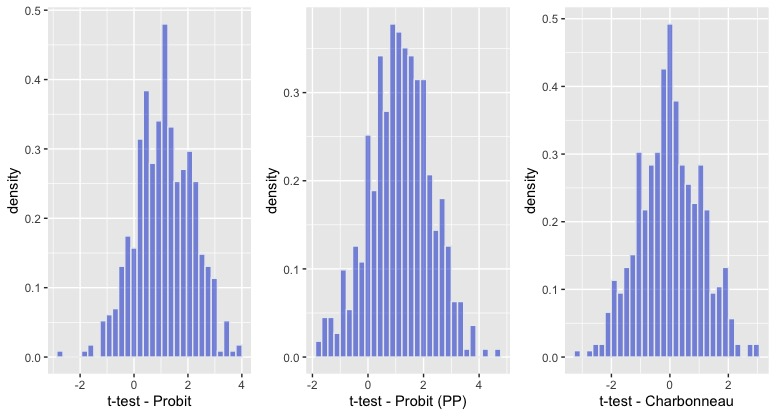
\includegraphics[scale=.4]{content/Figures/ttest_beta22_Design5.png}}
    \caption{\footnotesize{Histogram of the \textit{t-test} for estimated $\beta_{22}^*$ in Design 5}}
    \label{ttest_beta22_Design5}
    \end{adjustwidth}
\end{figure}
\begin{figure}[htbp]
    \vspace{-2.5em}%
    \begin{adjustwidth}{-.5in}{-.5in}
    \centerline{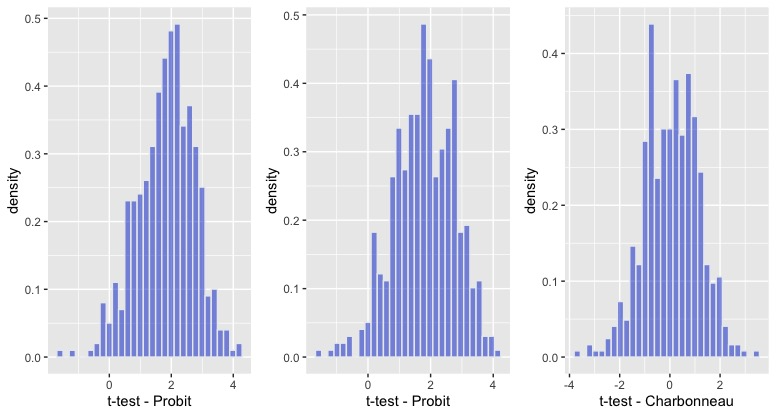
\includegraphics[scale=.4]{content/Figures/ttest_beta23_Design5.png}}
    \caption{\footnotesize{Histogram of the \textit{t-test} for estimated $\beta_{23}^*$ in Design 5}}
    \label{ttest_beta23_Design5}
\end{adjustwidth}
\end{figure}
\begin{figure}[htbp]
    \vspace{-2.5em}%
    \begin{adjustwidth}{-.5in}{-.5in}
    \centerline{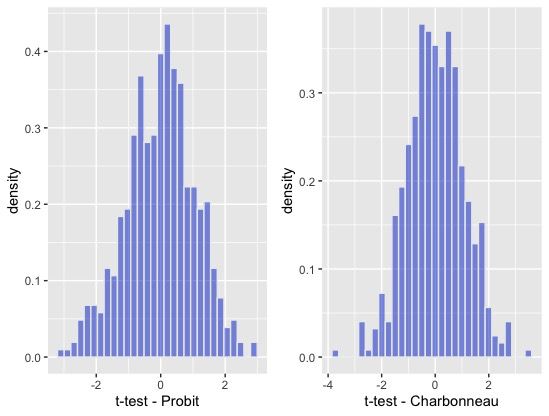
\includegraphics[scale=.4]{content/Figures/ttest_beta22_Design6.png}}
    \caption{\footnotesize{Histogram of the \textit{t-test} for estimated $\beta_{22}^*$ in Design 6}}
    \label{fittest_beta22_Design6g}
\end{adjustwidth}
\end{figure}
\begin{figure}[htbp]
    \vspace{-2.5em}%
    \begin{adjustwidth}{-.5in}{-.5in}
    \centerline{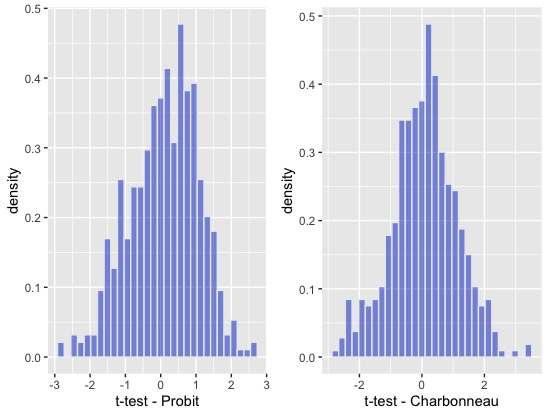
\includegraphics[scale=.4]{content/Figures/ttest_beta23_Design6.png}}
    \caption{\footnotesize{Histogram of the \textit{t-test} for estimated $\beta_{23}^*$ in Design 6}}
    \label{ttest_beta23_Design6}
\end{adjustwidth}
\end{figure}
\begin{figure}[htbp]
    \vspace{-2.5em}%
    \begin{adjustwidth}{-.5in}{-.5in}
    \centerline{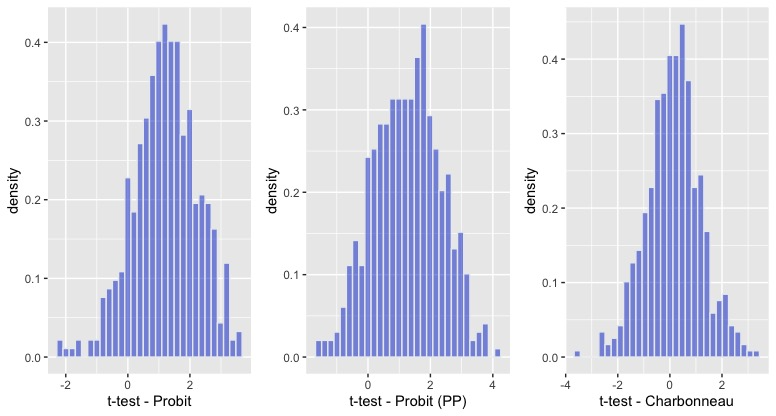
\includegraphics[scale=.4]{content/Figures/ttest_beta22_Design7.png}}
    \caption{\footnotesize{Histogram of the \textit{t-test} for estimated $\beta_{22}^*$ in Design 7}}
    \label{ttest_beta22_Design7}
\end{adjustwidth}
\end{figure}
\begin{figure}[htbp]
    \vspace{-2.5em}%
    \begin{adjustwidth}{-.5in}{-.5in}
    \centerline{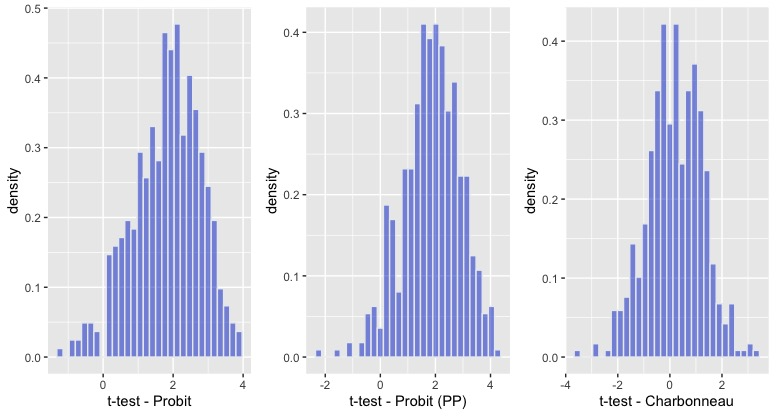
\includegraphics[scale=.4]{content/Figures/ttest_beta23_Design7.png}}
    \caption{\footnotesize{Histogram of the \textit{t-test} for estimated $\beta_{23}^*$ in Design 7}}
    \label{ttest_beta23_Design7}
\end{adjustwidth}
\end{figure}
\begin{figure}[htbp]
    \vspace{-2.5em}%
    \begin{adjustwidth}{-.5in}{-.5in}
\centerline{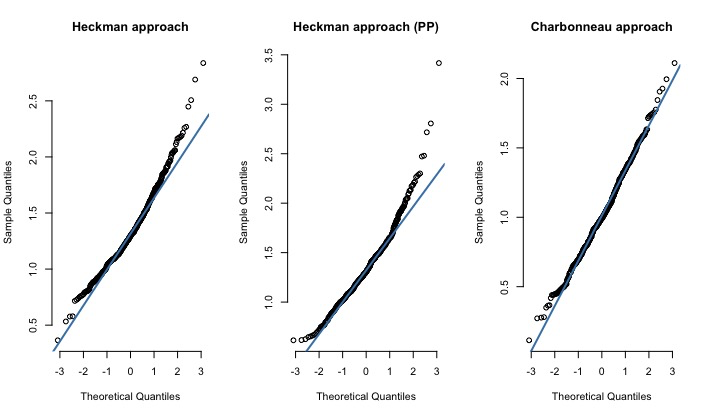
\includegraphics[scale=.4]{content/Figures/QQ_beta_22_Design5.png}}
\caption{\footnotesize{QQ plot of estimated $\beta_{22}^*$ in Design 5}}
\label{QQ_beta_22_Design5}
\end{adjustwidth}
\end{figure}
\begin{figure}[htbp]
    \vspace{-2.5em}%
    \begin{adjustwidth}{-.5in}{-.5in}
\centerline{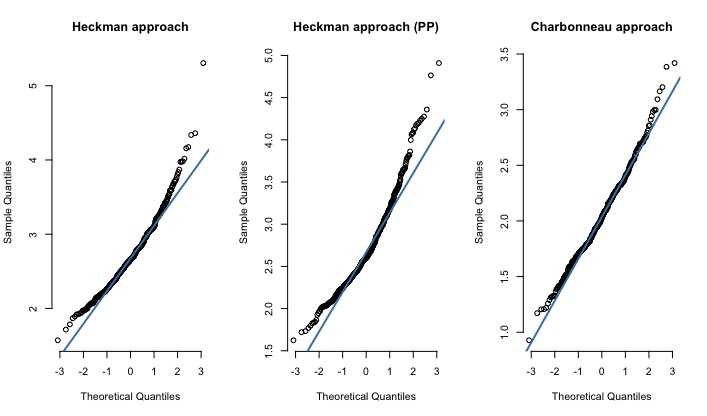
\includegraphics[scale=.4]{content/Figures/QQ_beta_23_Design5.png}}
\caption{\footnotesize{QQ plot of estimated $\beta_{23}^*$ in Design 5}}
\label{QQ_beta_23_Design5}
\end{adjustwidth}
\end{figure}
\begin{figure}[htbp]
    \vspace{-2.5em}%
    \begin{adjustwidth}{-.5in}{-.5in}
\centerline{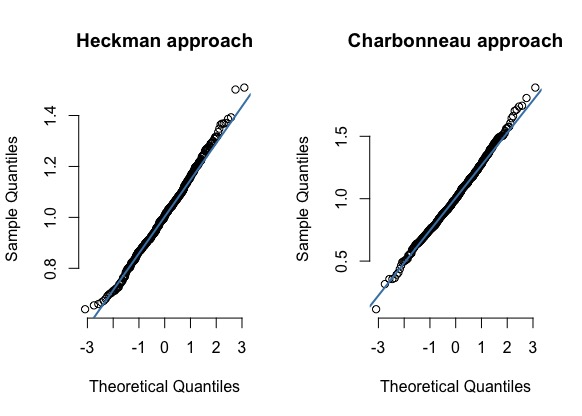
\includegraphics[scale=.4]{content/Figures/QQ_beta_22_Design6.png}}
\caption{\footnotesize{QQ plot of estimated $\beta_{22}^*$ in Design 6}}
\label{QQ_beta_22_Design6}
\end{adjustwidth}
\end{figure}
\begin{figure}[htbp]
    \vspace{-2.5em}%
    \begin{adjustwidth}{-.5in}{-.5in}
\centerline{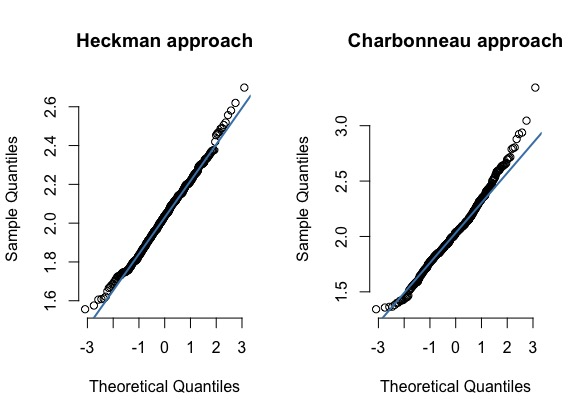
\includegraphics[scale=.4]{content/Figures/QQ_beta_23_Design6.png}}
\caption{\footnotesize{QQ plot of estimated $\beta_{23}^*$ in Design 6}}
\label{QQ_beta_23_Design6}
\end{adjustwidth}
\end{figure}
\begin{figure}[htbp]
    \vspace{-2.5em}%
    \begin{adjustwidth}{-.5in}{-.5in}
    \centerline{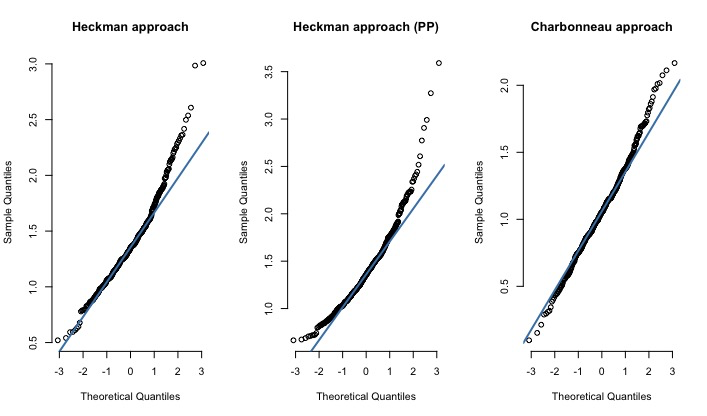
\includegraphics[scale=.4]{content/Figures/QQ_beta_22_Design7.png}}
    \caption{\footnotesize{QQ plot of estimated $\beta_{22}^*$ in Design 7}}
    \label{QQ_beta_22_Design7}
\end{adjustwidth}
\end{figure}
\begin{figure}[htbp]
    \vspace{-2.5em}%
    \begin{adjustwidth}{-.5in}{-.5in}
    \centerline{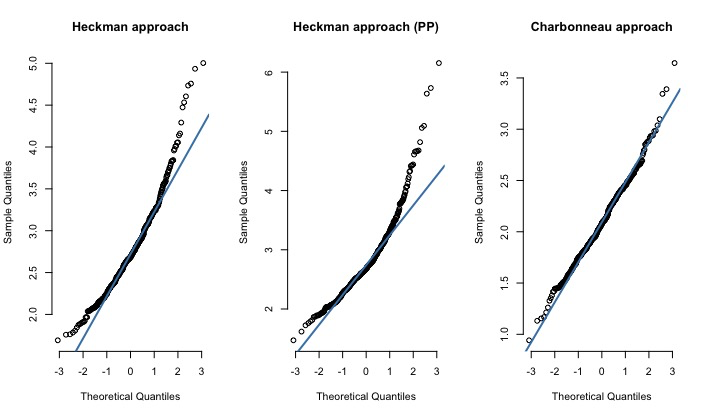
\includegraphics[scale=.4]{content/Figures/QQ_beta_23_Design7.png}}
    \caption{\footnotesize{QQ plot of estimated $\beta_{23}^*$ in Design 7}}
    \label{QQ_beta_23_Design7}
\end{adjustwidth}
\end{figure}
\clearpage
\subsection{Second stage estimates}
\begin{table}
    \begin{adjustwidth}{-.5in}{-.5in}
    \small
    \centering
    \begin{tabular}{p{3cm}p{1.3cm}p{1.3cm}p{1.3cm}p{1.3cm}p{1.3cm}p{1.3cm}p{1.3cm}}
      \hline
       \quad & Design 1 & Design 2 & Design 3 & Design 4 & Design 5 & Design 6 & Design 7  \\
       \hline
       \multicolumn{8}{l}{Hybrid} \\
       \hline
        $\beta_{11}$  & -0.0052 (0.0569) & 0.0000 (0.0747) & 0.0001 (0.0672) & 0.0014 (0.0750) & 0.0014 (0.0893) & 0.0033 (0.0745) & 0.0001 (0.0963) \\
        $\beta_{12}$  & 0.0022 (0.0821) & 0.0042 (0.1336) & 0.0041 (0.1263) & -0.0188 (0.1426) & -0.0026 (0.1547) & 0.0036 (0.1313) & -0.0194 (0.1680)\\
        Inverse Mills-Ratio  &  0.0013 (0.1306) & 0.0036 (0.2508) & 0.0143 (0.2524) & -0.0112 (0.2738)  & 0.0155 (0.3001) & 0.0212 (0.2627) & -0.0030
    (0.2977)\\
         & & & & & & & \\
        \hline
        \multicolumn{8}{l}{Kyriazidou $h=0.5$} \\
       \hline
        $\beta_{11}$  & -0.0054 (0.0759) & 0.0011 (0.0831) & -0.0060 (0.0779) & -0.0046 (0.0837) & 0.0019 (0.0935) & -0.0018 (0.0837) & -0.0067 (0.0887)\\
        $\beta_{12}$  & -0.0010 (0.1305) & -0.0032 (0.1401) & -0.0022 (0.1304) & -0.0082 (0.1431) & 0.0075 (0.1587) &  0.0056 (0.1391) & -0.0032 (0.1551) \\
         & & & & & & & \\
        \hline
        \multicolumn{8}{l}{Kyriazidou $h=0.5$, corrected} \\
       \hline
        $\beta_{11}$  & -0.0054 (0.0762) & 0.0011 (0.0834) & -0.0060 (0.0782) &  -0.0046 (0.0840) & 0.0019 (0.0939) & -0.0018 (0.0840) & -0.0068 (0.0890) \\
        $\beta_{12}$  & -0.0010 (0.1310) & -0.0033 (0.1407)  & -0.0023 (0.1309) & -0.0082 (0.1437) & 0.0074 (0.1593) & 0.0056 (0.1396) & -0.0031 (0.1558) \\
         & & & & & & & \\
        \hline
        \multicolumn{8}{l}{Kyriazidou $h=1$} \\
       \hline
        $\beta_{11}$  & -0.0061 (0.0685) & 0.0011 (0.0746) & -0.0057 (0.0697) & -0.0042 (0.0757) & 0.0000 (0.0841) &  -0.0029 (0.0743) & -0.0062 (0.0788) \\
        $\beta_{12}$  & 0.0001 (0.1161) & -0.0017 (0.1228) & -0.0013 (0.1162) & -0.0124 (0.1254) & 0.0090 (0.1403) &  0.0071 (0.1270) & -0.0083 (0.1361) \\
         & & & & & & & \\
            \hline
        \multicolumn{8}{l}{Kyriazidou $h=1$, corrected} \\
       \hline
        $\beta_{11}$  & -0.0062 (0.0687) & 0.0010 (0.0748) & -0.0058 (0.0699) & -0.0043 (0.0759) & 0.0000 (0.0843) &  -0.0030 (0.0745) & -0.0064 (0.0791) \\
        $\beta_{12}$  & 0.0001 (0.1164) & -0.0018 (0.1231) & -0.0015 (0.1165) & -0.0125 (0.1257) & 0.0090 (0.1407) &  0.0070 (0.1273) & -0.0083 (0.1364)\\
         & & & & & & & \\
        \hline
        \multicolumn{8}{l}{Kyriazidou $h=2$} \\
        \hline
         $\beta_{11}$  & -0.0063 (0.0647) & 0.0010 (0.0699) & -0.0048 (0.0641) & -0.0029 (0.0699) &-0.0012 (0.0785)  & -0.0036 (0.0686) & -0.0050 (0.0726)\\
         $\beta_{12}$  & 0.0000 (0.1098) & 0.0001 (0.1150) & 0.0000 (0.1097) & -0.0145 (0.1172) & 0.0084 (0.1324) & 0.0064 (0.1207) & -0.0103 (0.1256) \\
         & & & & & & & \\
         \hline
         \multicolumn{8}{l}{Kyriazidou $h=2$, corrected} \\
        \hline
         $\beta_{11}$  & -0.0066 (0.0649) & 0.0001 (0.0700) & -0.0052 (0.0643) & -0.0033 (0.0701) & -0.0014 (0.0787) &  -0.0040 (0.0688) & -0.0052 (0.0728) \\
         $\beta_{12}$  & 0.0000 (0.1100) & 0.0000 (0.1152) & -0.0001 (0.1099) & -0.0149 (0.1174) & 0.0082 (0.1327) &  0.0060 (0.1209) & -0.0106 (0.1258)\\
              & & & & & & & \\
         \hline
    \end{tabular}
    \caption{\footnotesize{Simulation results for the estimated coefficients for the observation Equation \ref{eq:dgp1} with $N=25$ and 500 iterations. For these results, we set the values of the parameters from the first stage Equation \ref{eq:dgp3} to be equal to their true values. The values correspond to the mean bias of estimates, and the standard deviation is in parenthesis.}}
    \label{tab:4}
    \end{adjustwidth}
\end{table}

\begin{table}
    \begin{adjustwidth}{-.5in}{-.5in}
    \small
    \centering
    \begin{tabular}{p{3cm}p{1.3cm}p{1.3cm}p{1.3cm}p{1.3cm}p{1.3cm}p{1.3cm}p{1.3cm}}
      \hline
       \quad & Design 1 & Design 2 & Design 3 & Design 4 & Design 5 & Design 6 & Design 7  \\
       \hline
        \multicolumn{8}{l}{Kyriazidou $h=3$} \\
       \hline
        $\beta_{11}$  & -0.0060 (0.0632) & 0.0011 (0.0685) & -0.0039 (0.0622) & -0.0019 (0.0675) & -0.0001 (0.0763) &  -0.0033 (0.0665) & -0.0038 (0.0700) \\
        $\beta_{12}$  & 0.0000 (0.1081) & 0.0019 (0.1128) & 0.0000 (0.1078) & -0.0139 (0.1146) & 0.0085 (0.1290) & 0.0065 (0.1176) & -0.0097 (0.1224) \\
        & & & & & & & \\
        \hline
        \multicolumn{8}{l}{Kyriazidou $h=3$, corrected} \\
       \hline
        $\beta_{11}$  & -0.0065 (0.0634) & 0.0001 (0.0686) & -0.0045 (0.0623) & -0.0024 (0.0677) & -0.0013 (0.0766) & -0.0038 (0.0667) & -0.0042 (0.0702)\\
        $\beta_{12}$  & 0.0000 (0.1083) & 0.0013 (0.1130) & 0.0000 (0.1080) & -0.0145 (0.1148) & 0.0081 (0.1293) &  0.0059 (0.1178) & -0.0101 (0.1226)\\
                 & & & & & & & \\
        \hline
        \multicolumn{8}{l}{Kyriazidou $h=5$} \\
       \hline
        $\beta_{11}$  & -0.0042 (0.0615) & 0.0020 (0.0672) & -0.0020 (0.0606) & 0.0001 (0.0649) & 0.0001 (0.0740) &  -0.0011 (0.0645) & -0.0015 (0.0673)\\
        $\beta_{12}$  & 0.0029 (0.1062) & 0.0040 (0.1103) & 0.0021 (0.1058) & -0.0117 (0.1123) & 0.0100 (0.1254) &  0.0082 (0.1141) & -0.0080 (0.1198) \\
        & & & & & & & \\
        \hline
        \multicolumn{8}{l}{Kyriazidou $h=5$, corrected} \\
       \hline
        $\beta_{11}$  & -0.0050 (0.0617) & 0.0014 (0.0674) & -0.0028 (0.0608) & 0.0000 (0.0651) & 0.0000 (0.0742) &  -0.0018 (0.0647) & -0.0020 (0.0675)\\
        $\beta_{12}$  & 0.0020 (0.1065) & 0.0032 (0.1106) & 0.0012 (0.1060) & -0.0125 (0.1125) & 0.0094 (0.1257) &  0.0073 (0.1143) & -0.0086 (0.1201) \\
                     & & & & & & & \\
        \hline
        \multicolumn{8}{l}{Kyriazidou $h=10$} \\
       \hline
        $\beta_{11}$  & 0.0046 (0.0583) & 0.0090 (0.0646) & 0.0070 (0.0578) & 0.0091 (0.0613) & 0.0067 (0.0702) &  0.0073 (0.0612) & 0.0050 (0.0637) \\
        $\beta_{12}$  & 0.0147 (0.1023) & 0.0128 (0.1074) & 0.0123 (0.1029) & -0.0026 (0.1090) & 0.0168 (0.1206) & 0.0180 (0.1096) & -0.0016 (0.1160)\\
        & & & & & & & \\
        \hline
        \multicolumn{8}{l}{Kyriazidou $h=10$, corrected} \\
       \hline
        $\beta_{11}$  & 0.0037 (0.0584) & 0.0083 (0.0648) & 0.0061 (0.0580) & 0.0083 (0.0615) & 0.0062 (0.0704) &  0.0065 (0.0614) & 0.0045 (0.0639)\\
        $\beta_{12}$  & 0.0136 (0.1025) & 0.0120 (0.1076) & 0.0112 (0.1031) & -0.0035 (0.1092) & 0.0162 (0.1208) & 0.0170 (0.1098) & -0.0022 (0.1162) \\
        \hline
    \end{tabular}
    \caption{\footnotesize{Simulation results for the estimated coefficients for the observation Equation \ref{eq:dgp1} with $N=25$ and 500 iterations. For these results, we set the values of the parameters from the first stage Equation \ref{eq:dgp3} to be equal to their true values. The values correspond to the mean bias of estimates, and the standard deviation is in parenthesis.}}
    \label{tab:5}
    \end{adjustwidth}
\end{table}
\begin{figure}[htbp]
    \begin{adjustwidth}{-.5in}{-.5in}
        \centerline{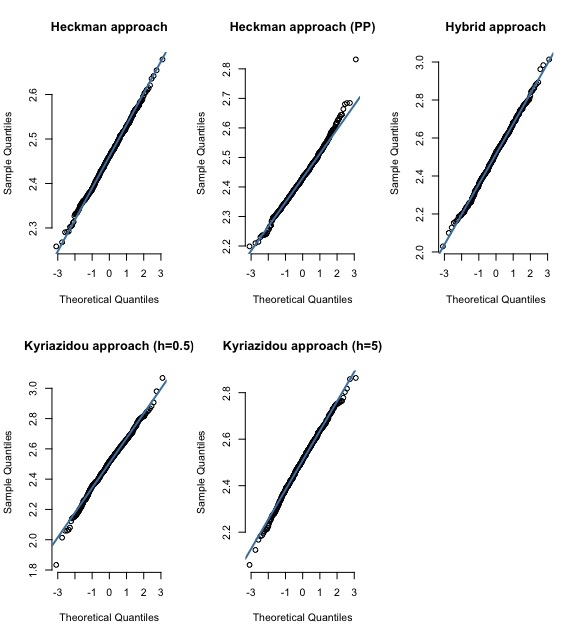
\includegraphics[scale=.4]{content/Figures/QQ_beta_12_Design5.png}}
        \caption{\footnotesize{QQ plot of estimated $\beta_{12}$ in Design 5}}
        \label{QQ_beta_12_Design5}
    \end{adjustwidth}
\end{figure}    
\begin{figure}[htbp]
    \vspace{-2.5em}%
    \begin{adjustwidth}{-.5in}{-.5in}
        \centerline{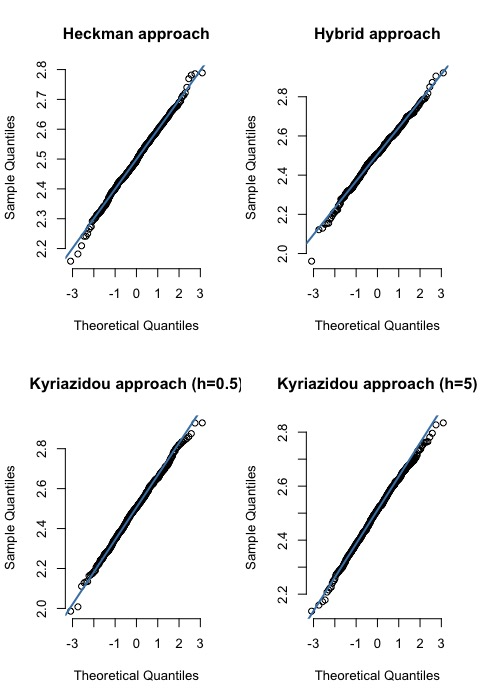
\includegraphics[scale=.4]{content/Figures/QQ_beta_12_Design6.png}}
        \caption{\footnotesize{QQ plot of estimated $\beta_{12}$ in Design 6}}
        \label{QQ_beta_12_Design6}
    \end{adjustwidth}
\end{figure}     
\begin{figure}[htbp]
    \vspace{-2.5em}%
    \begin{adjustwidth}{-.5in}{-.5in}
        \centerline{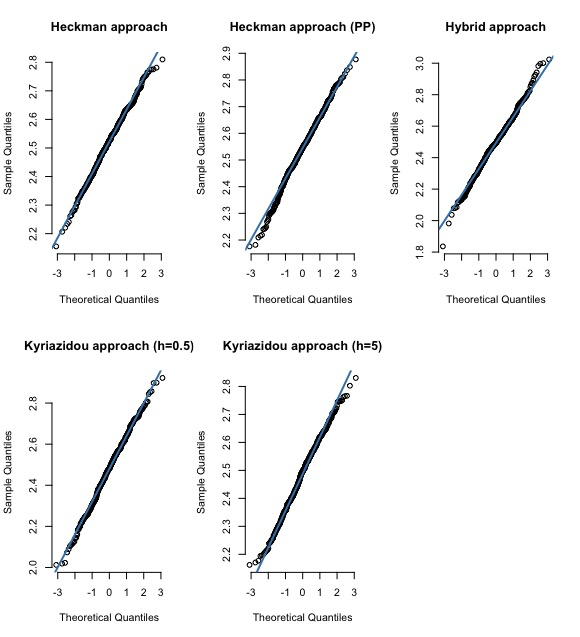
\includegraphics[scale=.4]{content/Figures/QQ_beta_12_Design7.png}}
        \caption{\footnotesize{QQ plot of estimated $\beta_{12}$ in Design 7}}
        \label{QQ_beta_12_Design7}
    \end{adjustwidth}
\end{figure}

